This chapter describes how the testbed was built and how the models were trained and evaluated. \Cref{sec:design-process} sets out the stage-gated design. \Cref{sec:preliminary-design} explains the alternatives we considered and the models we chose. \Cref{sec:data-collection} covers the data, from the BARC calendars to the hardened test set. \Cref{sec:implementation} covers training, inference, the metrics, the clarify-training intervention, the post-hoc detector, the human study and the statistical analysis plan.

\section{Design Process or Methodology Overview}
\label{sec:design-process}

The study was run as a sequence of stages, S0 to S8 (\cref{fig:pipeline}). Each stage wrote a gate report in machine-readable form, and the next stage began only after the report passed and had been reviewed. The stages were designed around one question: whether any number reported for the test set could have been inflated by the test set leaking into training. Five rules held throughout.

The first rule was to split before augmenting. The seed corpus was divided into training, validation and test sets before any row was generated, so that no generated row could be a variant of a held-out row. The second rule was that the held-out splits were never augmented and never opened by the augmentation code; the augmentation script refused, at run time, to open any file with a held-out name. The third rule was that the test set was locked: its SHA-256 hash was recorded after hardening and checked before every evaluation run and by every script that produced a number in this thesis. The fourth rule was never to impute: a calendar field with no recorded value produced no question at all. The fifth rule was to fix every source of randomness with a seed and to write every model output to disk before scoring it, so that any metric could be recomputed from the saved generations.

\section{Preliminary Design or Design (Model) Specification}
\label{sec:preliminary-design}

\subsection{Alternatives considered}
\label{sec:alternatives}

The project went through three designs. The first (v1) was an advisory application that retrieved calendar passages with a vector index, used a commercial LLM to read the farmer's question, and passed the extracted values to a deterministic calculator written in Python. The second (v2) replaced retrieval with a single fine-tuned model. Its corpus was generated first and split afterwards, so reworded versions of test questions were present in training, and its near-perfect held-out scores (\cref{sec:scope}) measured memorisation. The third design (v3), reported here, keeps the calculator as the source of every gold answer but asks the model to do the whole task: read a Bengali or English question, recall the crop coefficient, apply the effective-rainfall rule, compute the net depth and convert it to a volume.

Asking a model to do arithmetic that a Python function does perfectly needs a reason. Our reason is that the irrigation calculation is a controlled testbed, not the product. In any deployed system, even one that hands the arithmetic to a calculator or retrieves the coefficient table, a model still has to extract the inputs from the farmer's question. A model that invents a missing input will pass the invented value to the calculator, and nothing downstream can tell that it was invented. The calculation gives us an exact gold answer for every complete question and a precise definition of what is missing from every incomplete one. That makes the behaviour we study measurable.

A fourth design was considered and not run before this thesis was compiled: a prompted baseline, in which the base models receive an explicit system prompt with the formula, the coefficient table and an instruction to ask for missing values, with and without fine-tuning. It would separate what fine-tuning teaches from what an instruction can achieve. It is part of the supplementary round (\STAGEEIGHTB{prompted baseline, arms $\times$ 4 models}).

\subsection{Model choice}
\label{sec:model-choice}

We chose four instruction-tuned, open-weight models that fit on one consumer GPU when quantised to 4 bits and that differ in size, architecture family and tokenizer (\cref{tab:models}): Llama-3.1-8B~\cite{grattafiori2024llama}, Mistral-NeMo-12B~\cite{mistral2024nemo}, Phi-3.5-mini~\cite{abdin2024phi3} and Phi-4-mini~\cite{microsoft2025phi4mini}. Llama and Mistral form a large tier and the two Phi models a small tier. We used the instruction-tuned checkpoints because an advisory system would start from one, and because their chat templates give the zero-shot and fine-tuned arms an identical prompt format.

\subsection{Adapter configuration}
\label{sec:adapter-config}

All models were fine-tuned with QLoRA~\cite{dettmers2023qlora}: the base weights were loaded in 4-bit NormalFloat (NF4) precision and frozen, and low-rank adapters~\cite{hu2022lora} of rank \LoraRank, scaling factor $\alpha = \LoraAlpha$ and dropout \LoraDropout were trained on every projection matrix of every decoder layer. For Llama, Mistral and Phi-3.5 this meant \LlamaLoraTargets target modules per layer (the query, key, value and output projections of attention and the gate, up and down projections of the feed-forward block). Phi-4-mini stores the query, key and value projections as one fused matrix and the gate and up projections as another, so the same paths are covered by \PhiFourLoraTargets modules. The adapters therefore have different parameter counts (\cref{tab:models}) and Phi-4-mini's adapter is not structurally identical to the others. A first attempt that used the seven-module list for Phi-4-mini attached adapters to only part of the network (\PhiFourBrokenAdapterParams trainable parameters); the preflight check caught this before training.

\section{Data Collection}
\label{sec:data-collection}

\subsection{Source and digitisation}
\label{sec:source}

The domain facts come from the BARC crop calendars~\cite{barc2026cropcalendar}. The project folder holds \CalendarImageFiles calendar image files. Of these, \CalendarImageUnique are distinct files (\CalendarImageDuplicates are byte-identical duplicate scans), and \CalendarImageOutsideStudy distinct named image shows a crop outside the study set, leaving the \SourceFiles calendars that were digitised into \CalendarJsonFiles structured files, one per crop. Each file records, for its crop, the sowing and planting window, the growth stages and their timing, the critical irrigation periods, fertiliser and pest notes, and the provenance of each field.

How the images were turned into structured files is only partly documented. An extraction script from the first version of the project, which read the images with a commercial vision model, exists in the repository, but no record states whether a person checked every extracted value against its image. A digitisation check, in which two people independently compare a sample of extracted facts with the images, is part of the supplementary round (\STAGEEIGHTB{digitisation check}). Until it is done, the extracted facts are treated as the ground truth of the testbed and their error rate is unknown.

The crop coefficients come from a separate table with \KcRows rows. The table's own source column attributes \KcRowsFao rows to Table 12 of FAO-56~\cite{allen1998fao56} and \KcRowsIslam rice rows to a field study of rice in Bangladesh, while its citation column names an earlier FAO paper by Doorenbos and Pruitt for \KcFaoRowsCitingDoorenbos of the rows labelled FAO-56. BARC calendars give stages and irrigation timing, not coefficients, so these values did not come from the calendars, and their attribution has not been checked against the sources (\STAGEEIGHTB{crop-coefficient provenance}). This matters for interpretation: the coefficient table is a convention of this system, and what the models learn is that convention.

\subsection{Seed corpus}
\label{sec:seed-corpus}

From the structured calendars we built a seed corpus with exactly one canonical question per fact and language (stage S0). This gave \SeedRows rows covering \SeedFacts facts across \SeedCrops crops, with exactly \SeedRowsBn in Bengali and \SeedRowsBn in English. Each answer came from one of three sources. A retrieved answer is a verified field value, or a fixed composition of field values, with no wording invented beyond connecting text (\SeedFactual factual rows). A computed answer is produced by the irrigation calculator for a numeric scenario (\SeedNumeric numeric rows). An abstain answer is a refusal to a question outside the calendar's scope, such as market prices (\SeedAbstain rows). Fields marked as absent, excluded or needing review produced no question; \SeedSkippedInstances field instances of \SeedSkippedFieldTypes types were skipped and logged rather than guessed.

\subsection{Data Cleaning}
\label{sec:cleaning}

Bengali text needs normalisation before two strings can be compared, because the same word can be typed with different Unicode sequences. The first normaliser used for comparisons in the project removed combining vowel signs (matras) along with other marks, so that distinct Bengali words compared equal. Version 3.1, used from Stage 2 onward, preserves vowel signs and was checked against \BnNormCases test cases at the entry gate of every evaluation run. A second fault appeared during evaluation: the normaliser also removed decimal points, which destroyed every decimal number in a Bengali answer. Numeric parsing was therefore given its own digit transliteration (Bengali digits to ASCII digits, nothing else changed), and text normalisation was used only for text metrics.

\subsection{Data Transformation}
\label{sec:transformation}

Every row was rendered as a single-turn chat: the question as the user turn and the gold answer as the assistant turn, formatted with each model's own chat template. No system prompt was used. During training the loss was computed on the answer tokens only, and a masking gate checked on \MaskingProbes real examples that the prompt tokens were excluded. At evaluation the zero-shot arms received exactly the same prompt as the fine-tuned arms, so the only difference between arms was the weights. This also means the base models were never told the formula, the coefficient table or that they could ask for a missing value. We return to this limitation in \cref{sec:threats}.

\subsection{Data Integration}
\label{sec:integration}

Every numeric gold answer was computed by one function, the irrigation calculator, which the corpus builder, the test-hardening script and the evaluation all import. For a crop at growth stage $s$ with reference evapotranspiration $\mathrm{ET}_0$ (mm), rainfall $R$ (mm) and field area $A$ (m\textsuperscript{2}), the calculator computes
\begin{align}
  \mathrm{ET}_c &= K_c(s) \times \mathrm{ET}_0, \label{eq:etc}\\
  P_\mathrm{eff}(R) &= \begin{cases}
      \RainFactorOne \, R & R \le \RainTierOneMax\,\text{mm},\\
      \RainFactorTwo \, R & \RainTierOneMax\,\text{mm} < R \le \RainTierTwoMax\,\text{mm},\\
      \RainFactorThree \, R & R > \RainTierTwoMax\,\text{mm},
  \end{cases} \label{eq:peff}\\
  d &= \max\left(\mathrm{ET}_c - P_\mathrm{eff}(R),\, 0\right), \label{eq:net}\\
  V &= d \times A \quad \text{(litres, with $d$ in mm and $A$ in m\textsuperscript{2})}. \label{eq:volume}
\end{align}
Equation \eqref{eq:etc} is the FAO-56 crop-coefficient method~\cite{allen1998fao56}. The tiered effective-rainfall rule in \eqref{eq:peff} is this project's convention; it is not taken from FAO-56 or from BARC. The coefficient $K_c(s)$ is read from the table described in \cref{sec:source}, which has one column for each of \KcStages stages (initial, mid-season and late-season); FAO-56's crop-development stage has no column and is never asked about. Field sizes in local units are converted with fixed factors: an acre is \AreaAcre\,m\textsuperscript{2}, a bigha \AreaBigha\,m\textsuperscript{2}, a katha \AreaKatha\,m\textsuperscript{2}, a decimal \AreaDecimal\,m\textsuperscript{2} and a hectare \AreaHectare\,m\textsuperscript{2}. The bigha varies by region in Bangladesh, which the test set exploits.

The original design intended every net depth to be clamped to per-crop minimum and maximum bounds taken from BARC. The file of bounds was never written. Rather than invent bounds, the calculator applies only the physical floor in \eqref{eq:net} and records that no clamp was applied. All gold answers are therefore unclamped, and a gold depth of zero is common: \ZeroGoldPct\% of the single-crop numeric test rows (\ZeroGoldN of \NumericSingle) have a gold depth of zero, because effective rainfall exceeds crop water use.

\subsection{Data Splitting, Augmentation and Leakage Audit}
\label{sec:splitting}

This subsection replaces the template's ``Data Reduction'', which does not apply to this study.

\subsubsection*{Split first}
The seed corpus was split at stage S1 with a grouped shuffle split: every source group, which holds the Bengali and English rows of one fact, went wholly into one split, with target proportions of \SplitRatioTrain\%, \SplitRatioVal\% and \SplitRatioTest\% stratified by question type, language and crop. This produced \TrainSeedRows training, \ValRows validation and \TestSeedRows test rows. No source group, fact identifier or numeric scenario appears in more than one split (overlap counts \SplitOverlapSource, \SplitOverlapFact and \SplitOverlapScenario). The test split was hashed at this point.

\subsubsection*{Augment the training split only}
Stage S2 planned \AugFamiliesPlanned augmentation families. Two, paraphrase (A) and back-translation (B), needed calls to an external LLM and were never run, because no API key was available. The two that ran need no external model (\cref{tab:augmentation}). Family C generated \AugRowsSynthetic new numeric scenarios with gold answers from the calculator. It drew $\mathrm{ET}_0$ and rainfall independently (Pearson correlation \AugPearsonR, against a tolerance of \AugPearsonTol), allowed at most \AugZeroQuotaPct\% of scenarios to have a zero gold depth, and rejected any scenario whose hash appeared in a blocklist of the \AugBlocklistHashes held-out scenario hashes. The blocklist was exported by a separate script, so the augmentation code never read a held-out file. Family D added character-level typing noise to crop and unit words (\AugNoiseMade rows made, \AugDropBalance removed to keep the languages exactly balanced). The training corpus has \AugRows rows: \TrainPctNumeric\% numeric, \TrainPctFactual\% factual, \TrainPctAbstain\% abstain and \TrainPctClarify\% clarification. Most of it is synthetic numeric text from the same generator style as the numeric test rows, which creates a risk that numeric accuracy reflects template matching; we never describe the models' numeric behaviour as reasoning.

\subsubsection*{Leakage audit}
Stage S3 compared every augmented training row with every validation and test row using four detectors (\cref{tab:leakage}). The exact-match detector found \LeakExactCount identical normalised questions. The scenario detector found \LeakScenarioOverlap of the \LeakScenarioHeldout held-out numeric scenarios in training. The lexical detector flags pairs whose character 5-gram Jaccard similarity is at least \LeakJaccardThreshold. It found \LeakJaccardPairs such pairs, because all questions share templates. The original rule failed the audit on \LeakJaccardHitsOriginal pairs; after the rule was refined to fail only pairs that also share a fact identifier and are not abstain boilerplate (\LeakJaccardAbstainExcluded abstain pairs were excluded), \LeakJaccardHitsRefined pairs remained. These pairs ask about the same crop--stage fact with a different scenario. They were accepted as a documented limitation: the model may have seen the coefficient for a test crop and stage in training, but never the same inputs. The semantic detector, which compares multilingual sentence embeddings~\cite{reimers2020making} with FAISS~\cite{johnson2021billion}, flagged \LeakSemCandidates pairs with cosine similarity of at least \LeakSemThreshold for human review. The gate passed with \LeakSemDecisionsRecorded human decisions recorded, which it should not have. A review sample of \LeakReviewSample pairs has since been drawn with a fixed seed from the \LeakReviewFrame pairs stored in the audit report; because the report stores only the most similar pairs, the sample over-represents them. Its result is \PENDINGREVIEW{semantic leakage review, \LeakReviewSample pairs, two reviewers}. We therefore call the corpus leakage-audited, with these limits.

\subsection{Test Hardening}
\label{sec:hardening}

The seed test split comes from the same generator as the training corpus, so a fine-tuned model can score near its ceiling on it without handling any real difficulty. Stage S4 added \TestRowsAdv adversarial rows in seven categories, half Bengali and half English (\cref{tab:hardening}), giving a hardened test set of \TestRows rows, which was then hashed and locked. Every numeric gold was computed by the calculator, and every new scenario was checked against the training and held-out scenario hashes (\AdvScenarioCollisions collisions).

Three categories introduce incomplete questions and define the clarification probe. Missing-parameter rows omit one of $\mathrm{ET}_0$, rainfall, field area or growth stage (\AdvMissingEt rows each). Some misspelled-crop rows are ambiguous between two crops, for example between varieties of rice. Some unit-ambiguity rows state the field size in a local unit such as kani, whose size varies and is not in the conversion table. For all of these, the correct response is to ask for the missing or ambiguous value, and they are labelled with a new question type, clarify. The clarify type does not occur in the training corpus. We added it to the test set because we wanted to observe what fine-tuning does when no training example shows the right behaviour; the probe is part of the design, and its absence from training is by construction.

Two categories have no gold answer that a script can check. For conflicting-value questions, where a farmer states two different values, it is a policy choice whether to ask, take the later value or answer both ways. For adversarial out-of-domain questions, the boundary of the calendar's scope and the wording of a refusal are also policy. The \TestExcluded rows in these categories (\TestExcludedConflict conflicting, \TestExcludedOOD out-of-domain) were marked as awaiting a human-written gold and excluded from scoring by design. The scored test set therefore has \TestScorable rows: \TestNumeric numeric (\NumericSingle single-crop and \NumericMulti multi-crop), \TestFactual factual, \TestClarify clarify and \TestAbstain abstain, each split equally between the languages. Abstention is measured on the \TestAbstain seed out-of-domain rows only, which are easier than the excluded adversarial ones; scoring the excluded rows by class is part of the supplementary round (\STAGEEIGHTB{class-level scoring of the \TestExcluded excluded rows}).

\subsection{Summary of Preprocessed Data}
\label{sec:data-summary}

\Cref{tab:data} gives the rows at each stage and \cref{fig:data} shows the composition. The central fact of the design is visible in \cref{fig:data}(b): clarification is \TrainPctClarify\% of the training corpus but \TestPctClarifyScorable\% of the scored test set, while abstention is \TrainPctAbstain\% of training.

% AUTO-GENERATED by scripts/thesis/tables.py
\begin{table}[tbp]
\centering
\small
\caption{Dataset and split statistics. Rows by stage and question type. The seed corpus was split by source group before any augmentation; each source group holds one Bengali and one English row. Clarification rows exist only in the hardened test set and in the clarify-augmented corpus.}
\label{tab:data}
\begin{tabular}{lrrrrrr}
\toprule
Stage & Rows & Groups & Numeric & Factual & Abstain & Clarify \\
\midrule
Seed corpus (S0) & \SeedRows{} & \SeedSourceIds{} & \SeedNumeric{} & \SeedFactual{} & \SeedAbstain{} & -- \\
\quad train split (S1) & \SplitTrainSeedRows{} & \SplitTrainSeedGroups{} & \SplitTrainSeedNumeric{} & \SplitTrainSeedFactual{} & \SplitTrainSeedAbstain{} & -- \\
\quad validation split (S1) & \SplitValRows{} & \SplitValGroups{} & \SplitValNumeric{} & \SplitValFactual{} & \SplitValAbstain{} & -- \\
\quad test split (S1) & \SplitTestSeedRows{} & \SplitTestSeedGroups{} & \SplitTestSeedNumeric{} & \SplitTestSeedFactual{} & \SplitTestSeedAbstain{} & -- \\
\addlinespace
Training corpus (S2) & \AugRows{} & -- & \TrainNumeric{} & \TrainFactual{} & \TrainAbstain{} & \TrainClarify{} \\
Clarify-augmented corpus (S6B) & \ClarifyCorpusRows{} & -- & \TrainNumeric{} & \TrainFactual{} & \TrainAbstain{} & \ClarifyTrainRows{} \\
\addlinespace
Hardened test set (S4), all rows & \TestRows{} & -- & \TestAllNumeric{} & \TestAllFactual{} & \TestAllAbstain{} & \TestAllClarify{} \\
Hardened test set, scored rows & \TestScorable{} & -- & \TestNumeric{} & \TestFactual{} & \TestAbstain{} & \TestClarify{} \\
\bottomrule
\end{tabular}
\end{table}

% AUTO-GENERATED by scripts/thesis/tables.py
\begin{table}[tbp]
\centering
\small
\caption{Augmentation families. Families A and B required calls to an external language model and were not run; the training corpus comes from the seed rows plus families C and D. Family D produced \AugNoiseMade{} rows, of which \AugDropBalance{} were removed to keep the two languages exactly balanced.}
\label{tab:augmentation}
\begin{tabular}{c>{\raggedright\arraybackslash}p{0.5\textwidth}lr}
\toprule
Family & Method & Status & Rows kept \\
\midrule
A & Paraphrase of seed questions by an external LLM & not run & -- \\
B & Back-translation through the other language & not run & -- \\
C & Synthetic numeric scenarios, gold from \texttt{irrigation\_calc} & run & \AugRowsSynthetic{} \\
D & Character noise in crop and unit words & run & \AugRowsNoise{} \\
-- & Seed rows carried over unchanged & -- & \AugRowsSeed{} \\
\midrule
\multicolumn{3}{l}{Training corpus} & \AugRows{} \\
\bottomrule
\end{tabular}
\end{table}

% AUTO-GENERATED by scripts/thesis/tables.py
\begin{table}[tbp]
\centering
\footnotesize
\caption{Leakage detectors and outcomes (Stage 3), training corpus against the validation and test splits. The \LeakJaccardHitsRefined{} lexical pairs share a crop--stage fact but not a scenario; they were accepted as a documented limitation. The semantic detector passed with no human review recorded; the reviewed rate is \PENDINGREVIEW{semantic leakage sample}.}
\label{tab:leakage}
\begin{tabular}{>{\raggedright\arraybackslash}p{0.13\textwidth}>{\raggedright\arraybackslash}p{0.22\textwidth}l>{\raggedright\arraybackslash}p{0.3\textwidth}l}
\toprule
Detector & Signal & Threshold & Finding & Verdict \\
\midrule
Exact & identical normalised question & -- & \LeakExactCount{} pairs & pass \\
Lexical & character 5-gram Jaccard & \LeakJaccardThreshold{} & \LeakJaccardPairs{} pairs above threshold; \LeakJaccardHitsRefined{} under the refined rule & pass \\
Semantic & multilingual MiniLM cosine & \LeakSemThreshold{} & \LeakSemCandidates{} candidates; \LeakSemDecisionsRecorded{} reviewed & pass, unreviewed \\
Scenario & shared scenario hash & -- & \LeakScenarioOverlap{} of \LeakScenarioHeldout{} held-out hashes & pass \\
\bottomrule
\end{tabular}
\end{table}

% AUTO-GENERATED by scripts/thesis/tables.py
\begin{table}[tbp]
\centering
\footnotesize
\caption{Test hardening categories (Stage 4). Each category is half Bengali and half English. The two unscored categories (\TestExcluded{} rows) have no machine-verifiable gold answer and were excluded by design, so conflicting-value behaviour is not evaluated and abstention is measured on seed rows only.}
\label{tab:hardening}
\begin{tabular}{>{\raggedright\arraybackslash}p{0.16\textwidth}r>{\raggedright\arraybackslash}p{0.19\textwidth}>{\raggedright\arraybackslash}p{0.36\textwidth}l}
\toprule
Category & Rows & Question type & Subtypes & Scored \\
\midrule
Misspelled crop & \AdvMisspelled{} & \AdvMisspelledNumeric{} numeric, \AdvMisspelledClarify{} clarify & recoverable (\AdvMisspelledSubRecoverable{}), ambiguous (\AdvMisspelledSubAmbiguous{}) & yes \\
Missing parameter & \AdvMissingParam{} & \AdvMissingParamClarify{} clarify & ET0, rainfall, area, stage (\AdvMissingEt{} each) & yes \\
Unit ambiguity & \AdvUnitAmbig{} & \AdvUnitAmbigNumeric{} numeric, \AdvUnitAmbigClarify{} clarify & unknown local unit (\AdvUnitAmbigSubUnknownLocalUnit{}), regional bigha (\AdvUnitAmbigSubBighaRegional{}), stated conversion (\AdvUnitAmbigSubExplicitLocalConversion{}) & yes \\
Multi-crop & \AdvMultiCrop{} & \AdvMultiCropNumeric{} numeric & two answers (\AdvMultiCropSubDualAnswer{}), comparison (\AdvMultiCropSubComparative{}), split area (\AdvMultiCropSubSplitArea{}) & yes \\
Code-switched & \AdvCodeSwitched{} & \AdvCodeSwitchedNumeric{} numeric & \AdvCodeSwitchedSubtypes{} matrix-language variants & yes \\
Conflicting values & \AdvConflicting{} & \AdvConflictingClarify{} clarify & restated or contradicted inputs & no \\
Out of domain & \AdvOutOfDomain{} & \AdvOutOfDomainAbstain{} abstain & \AdvOutOfDomainSubtypes{} topics absent from training & no \\
\midrule
Adversarial total & \TestRowsAdv{} & & & \\
\bottomrule
\end{tabular}
\end{table}


\begin{figure}[tbp]
  \centering
  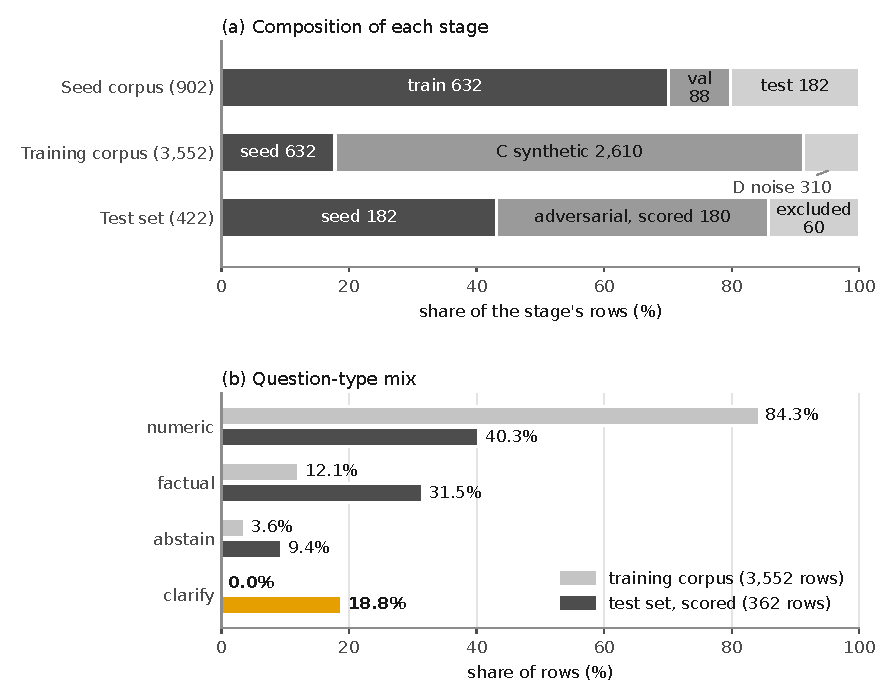
\includegraphics[width=\textwidth]{f02_data_composition}
  \caption{Data composition. (a) Rows of the seed corpus (\SeedRows), the training corpus (\AugRows) and the hardened test set (\TestRows) by origin. (b) Share of each question type in the training corpus and in the \TestScorable scored test rows. Clarification is absent from training (\TrainPctClarify\%) but is \TestPctClarifyScorable\% of the scored test set; abstention is \TrainPctAbstain\% of training.}
  \label{fig:data}
\end{figure}

\FloatBarrier

\section{Implementation of Selected Design}
\label{sec:implementation}

\subsection{Training}
\label{sec:impl-training}

Each of the four models was fine-tuned three times, with seeds 42, 1337 and 2024, on the same \AugRows-row corpus: twelve training runs (four models $\times$ three seeds). The seeds change the adapter initialisation, the data order and dropout; the data and the base weights are shared, so the seeds measure training randomness only, and the twelve runs are not twelve independent samples. Training used the settings in \cref{tab:hyperparameters} on a single \GpuName, through the Unsloth~\cite{unsloth2024}, TRL~\cite{trl2020} and Transformers~\cite{wolf2020transformers} libraries. The twelve runs took \TrainGpuHoursTwelve GPU-hours in total and none failed.

Every run used a fixed budget of \HpEpochs epochs with no early stopping. The validation split is not a good guide for early stopping here: it is \ValPctFactual\% factual and \ValPctNumeric\% numeric, while the training corpus is \TrainPctNumeric\% numeric, because augmentation added numeric rows only to the training side. \Cref{fig:training} shows that validation loss reached its minimum before the final step in \EvalMinBeforeFinalRuns of the twelve runs and ended at most \EvalRiseMax above that minimum. We used the final checkpoints, as fixed in advance. Phi-3.5-mini's validation loss was still falling late in training (its seed 42 minimum is at step \PhiThreeSeedAEvalMinStep), so it may be under-trained relative to the other models. Validation losses cannot be compared across models, because each tokenizer splits the same text into a different number of tokens. \Cref{fig:tokenizer} shows how large that difference is for Bengali: a Bengali question costs \RangeTokRatioMin to \RangeTokRatioMax times as many tokens as its English twin, depending on the tokenizer, in line with earlier findings that tokenizers treat languages unequally~\cite{petrov2023language,ahia2023all}.

Each run wrote a manifest with its settings, losses, adapter path and adapter SHA-256. The evaluation script was meant to check these manifests before loading an adapter, but in \ManifestCheckSkippedRuns evaluation runs the check was skipped by a command-line flag. We therefore re-verified every adapter afterwards: all \AdapterArmsPass of the \AdapterArms fine-tuned and clarify-trained arms loaded an adapter whose hash matches its manifest, and every zero-shot arm loaded base weights only.

% AUTO-GENERATED by scripts/thesis/tables.py
\begin{table}[tbp]
\centering
\footnotesize\setlength{\tabcolsep}{4pt}
\caption{Models and adapters. Targets are the projection modules that receive a LoRA adapter; every decoder layer is adapted. Phi-4-mini exposes fused query--key--value and gate--up projections, so its adapter covers the same paths through fewer, fused modules. Trainable parameters are in millions and identical across seeds. Peak VRAM is the maximum over three seeds; time is the mean training time per run on one \GpuName{}.}
\label{tab:models}
\begin{tabular}{llrrrrr}
\toprule
Model & Checkpoint & Targets & Layers & \makecell{Trainable\\ parameters (M)} & \makecell{VRAM\\ (GB)} & Minutes \\
\midrule
Llama-3.1-8B & \makecell[l]{\texttt{meta-llama/}\\\texttt{Llama-3.1-8B-Instruct}} & \LlamaLoraTargets{} & \LlamaLoraLayersAdapted{} & \LlamaTrainableParamsM{} & \LlamaPeakVramMax{} & \LlamaWallMinMean{} \\
Mistral-NeMo-12B & \makecell[l]{\texttt{mistralai/}\\\texttt{Mistral-Nemo-Instruct-2407}} & \MistralLoraTargets{} & \MistralLoraLayersAdapted{} & \MistralTrainableParamsM{} & \MistralPeakVramMax{} & \MistralWallMinMean{} \\
Phi-3.5-mini & \makecell[l]{\texttt{microsoft/}\\\texttt{Phi-3.5-mini-instruct}} & \PhiThreeLoraTargets{} & \PhiThreeLoraLayersAdapted{} & \PhiThreeTrainableParamsM{} & \PhiThreePeakVramMax{} & \PhiThreeWallMinMean{} \\
Phi-4-mini & \makecell[l]{\texttt{microsoft/}\\\texttt{Phi-4-mini-instruct}} & \PhiFourLoraTargets{} & \PhiFourLoraLayersAdapted{} & \PhiFourTrainableParamsM{} & \PhiFourPeakVramMax{} & \PhiFourWallMinMean{} \\
\bottomrule
\end{tabular}
\end{table}

% AUTO-GENERATED by scripts/thesis/tables.py
\begin{table}[tbp]
\centering
\small
\caption{Training and inference settings, identical for all four models except the per-device batch. Values are read from the training script and the run manifests.}
\label{tab:hyperparameters}
\begin{tabular}{l>{\raggedright\arraybackslash}p{0.55\textwidth}}
\toprule
Setting & Value \\
\midrule
Quantisation & 4-bit base weights, LoRA in bf16 \\
LoRA rank / alpha / dropout & \LoraRank{} / \LoraAlpha{} / \LoraDropout{} \\
Epochs & \HpEpochs{} (fixed; no early stopping) \\
Learning rate & $\HpLearningRate{}$, \HpScheduler{} schedule, \HpWarmup{} warm-up steps \\
Optimiser & \texttt{\HpOptim{}}, weight decay \HpWeightDecay{}, gradient clip \HpMaxGradNorm{} \\
Effective batch & \HpEffectiveBatch{} (per-device batch $\times$ accumulation) \\
\quad Llama / Mistral / Phi-3.5 / Phi-4 & \LlamaBatchSize{}$\times$\LlamaGradAccum{} / \MistralBatchSize{}$\times$\MistralGradAccum{} / \PhiThreeBatchSize{}$\times$\PhiThreeGradAccum{} / \PhiFourBatchSize{}$\times$\PhiFourGradAccum{} \\
Maximum sequence length & \MaxSeqLen{} tokens (longest training example \SeqLenGlobalMax{}) \\
Loss & completion tokens only (masking checked on \MaskingProbes{} examples) \\
Validation loss & every \HpEvalSteps{} steps, monitoring only \\
Seeds & 42, 1337, 2024 (clarify-trained models: 42 only) \\
Decoding & greedy, at most \GenMaxNewTokens{} new tokens \\
\bottomrule
\end{tabular}
\end{table}


\begin{figure}[tbp]
  \centering
  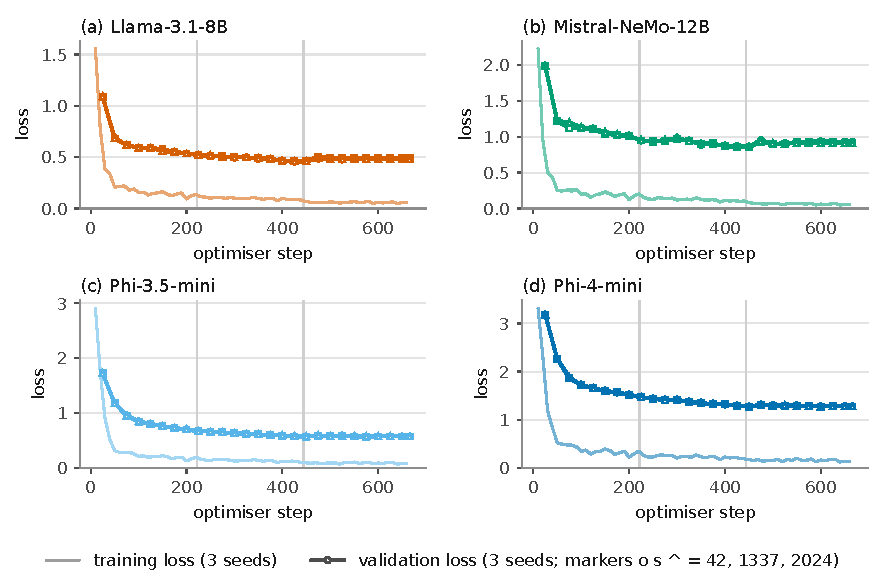
\includegraphics[width=\textwidth]{f04_training_dynamics}
  \caption{Training and validation loss for the twelve training runs, one panel per model; the three seeds share a colour and are marked o, s and \textasciicircum{} (seeds 42, 1337, 2024); vertical lines mark epoch boundaries. Training loss falls smoothly in every run. Validation loss reaches its minimum before the final step in \EvalMinBeforeFinalRuns of twelve runs and ends at most \EvalRiseMax above it. Validation loss is not comparable across models, because each tokenizer divides the same text into a different number of tokens.}
  \label{fig:training}
\end{figure}

\begin{figure}[tbp]
  \centering
  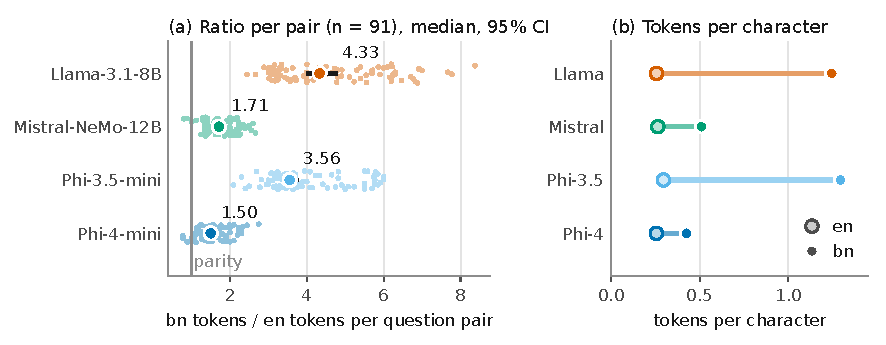
\includegraphics[width=\textwidth]{f03_tokenizer_cost}
  \caption{Tokenizer cost of Bengali. (a) Ratio of Bengali to English tokens for each of \TokPairs Bengali--English question pairs from the test set, with the median and its 95\% bootstrap CI. (b) Tokens per character in each language. A Bengali question costs \RangeTokRatioMin to \RangeTokRatioMax times as many tokens as its English twin; the cost is highest for Llama-3.1-8B and Phi-3.5-mini.}
  \label{fig:tokenizer}
\end{figure}

\subsection{Inference}
\label{sec:impl-inference}

All arms were evaluated on the locked test set with greedy decoding and at most \GenMaxNewTokens new tokens, with the base weights in 4-bit precision for every arm, so that zero-shot and fine-tuned arms differ only in the adapter. There are \EvalArms scored arms: four zero-shot, twelve fine-tuned and four clarify-trained, plus one arm that applies a post-hoc detector to the clarify-trained Llama outputs (\cref{sec:impl-detector}). Every generation was saved before any scoring. The inference code stores no finish reason, so whether a generation stopped at the token limit is inferred later by re-tokenising the saved text (\cref{sec:impl-plan}).

\subsection{Evaluation Metrics}
\label{sec:impl-metrics}

Each metric is defined for one question type and raises an error if applied to a row of another type, so no metric is ever averaged across types (\cref{tab:metrics}).

% AUTO-GENERATED by scripts/thesis/tables.py
\begin{table}[tbp]
\centering
\footnotesize
\caption{Metric definitions by question type. Each metric asserts the question type of the row it scores and raises an error on any other type, so no metric is averaged across types. Slot tolerances: Kc $\pm$\TolKc{}, ET0 and effective rainfall $\pm$\TolEt{} mm, area the larger of \TolAreaAbs{} m\textsuperscript{2} and \TolAreaRelPct{}\%.}
\label{tab:metrics}
\begin{tabular}{lr>{\raggedright\arraybackslash}p{0.3\textwidth}>{\raggedright\arraybackslash}p{0.36\textwidth}}
\toprule
Type & Rows & Headline metric & Other metrics \\
\midrule
Numeric & \TestNumeric{} & net depth within $\pm$0.1 mm (\NumericSingle{} single-crop rows; Stage 8 tests use all \NumericAll{} rows) & exact ($<$0.005 mm) and within $\pm$1.0 mm, always reported with the headline; MAE; RMSE; slot F1 for Kc, ET0, effective rainfall, area; both values correct on \NumericMulti{} multi-crop rows \\
Factual & \TestFactual{} & chrF++ & exact match; Dice; ROUGE-L; BERTScore F1 (unrescaled) \\
Clarify & \TestClarify{} & clarify exact: asks and names the missing parameter & learned clarification (asks, withholds the result); invented-value rate \\
Abstain & \TestAbstain{} & abstain accuracy & -- \\
\bottomrule
\end{tabular}
\end{table}
 For numeric rows, a parser extracts the stated net depth, crop coefficient, $\mathrm{ET}_0$, effective rainfall and area from the answer text in either language, and each is compared with the gold trace from the calculator. The headline numeric metric is the share of the \NumericSingle single-crop rows whose stated net depth lies within $\pm$0.1\,mm of the gold depth; this tolerance was fixed before results were seen. We always report it together with an exact tier (within 0.005\,mm, that is, equal after rounding to the two decimals the calculator uses) and a lenient tier (within $\pm$1.0\,mm). A row with no extractable depth counts as wrong. The \NumericMulti multi-crop rows need two depths and are scored separately. The statistical tests in Stage 8 use all \NumericAll numeric rows, counting a multi-crop row as correct only if every depth is within 0.1\,mm; since no arm got any multi-crop row fully right, this changes the denominator but not the count. Wherever an exact-match figure appears, we name its denominator. Slot F1 scores for the crop coefficient and the effective rainfall show whether a model has learned the system's conventions.

For factual rows the headline metric is chrF++~\cite{popovic2015chrf,popovic2017chrfpp}, computed with sacreBLEU~\cite{post2018call}; we also report exact match, word-level Dice, ROUGE-L~\cite{lin2004rouge} and BERTScore~\cite{zhang2020bertscore} computed with multilingual BERT~\cite{devlin2019bert} and not rescaled. The standard ROUGE implementation strips non-ASCII text and so reduced every Bengali reference to an empty string; we reimplemented ROUGE-L on the normalised tokens.

For clarify and abstain rows, a rule-based classifier assigns each response to one of four classes: answer, clarify, abstain or empty. It first looks for refusal phrases, then for request phrases (in both languages) such as ``please tell me'' or \bn{অনুগ্রহ করে}. A response that contains a request phrase but also delivers a complete result, a net depth and a volume in litres, is classed as an answer: a model that states litres for a field whose size was never given has invented the size. The primary clarify metric, \emph{clarify exact}, requires that the response asks and names the specific missing parameter (for example rainfall, field size or the unknown unit). A secondary metric, \emph{clarify learned}, counts any response classed as clarify. The \emph{invented-value rate} is the share of clarify rows whose response is classed as an answer. Abstain accuracy is the share of abstain rows classed as abstain.

\subsubsection*{Changes made after results were seen}

Three metric definitions were changed after the first Stage 6 results were known. Each change was checked with a gold-oracle arm, which scores the gold answers themselves and must reach \ChangeOracleAfter on every slot. First, slot scores were made not-applicable when the gold answer does not state the slot: only \ChangeCropCeilingPct\% of gold numeric answers name the crop and \ChangeStageCeilingPct\% name the stage, so scoring those slots against every row penalised correct answers. Second, the area tolerance was made relative (the larger of \TolAreaAbs\,m\textsuperscript{2} and \TolAreaRelPct\% of the gold area), because gold areas are converted from local units and an absolute tolerance was too strict for large fields. Third, half credit for a generic request that does not name the missing parameter was removed: every one of the \ChangeNamedNoAskPartials half-credit responses of the fine-tuned Llama at seed 42 was the worked-answer formula, which contains the words ``ET0'' and ``rainfall'', not a request. The oracle's score before these changes is not recorded in any file that survives, so we cannot report it; its score after them is \ChangeOracleAfter.

Two faults were fixed before any GPU time was spent on evaluation. A join between test rows and generations collapsed all \JoinBugCollapsed seed rows onto one key because their item identifier was empty. And \ChangeBighaGolds numeric gold answers that end with a courtesy sentence (``if a bigha is a different size in your area, tell me and I will recompute'') were classed as clarification requests until the classifier learned to treat a delivered result as an answer.

\subsection{Clarify-Training Intervention}
\label{sec:impl-clarify}

To test whether the missing behaviour can be taught, we built \ClarifyTrainRows clarification examples by deleting one input from numeric training rows and writing a templated request for it as the answer: \ClarifyTrainSlotRain each for rainfall, field area and growth stage, \ClarifyTrainBn in Bengali and \ClarifyTrainEn in English. No example deletes $\mathrm{ET}_0$ (\ClarifyTrainSlotEt rows), although the test set includes rows with $\mathrm{ET}_0$ missing, as well as ambiguous crops and unknown units, which the training examples never show. Adding these rows to the training corpus gave \ClarifyCorpusRows rows, of which \ClarifyCorpusPctClarify\% are clarification. Each model was retrained once, at seed 42, with the same settings as before. These clarify-trained models (CL) therefore exist at one seed only, and their comparison with the fine-tuned models uses the seed 42 fine-tuned runs.

\subsection{Post-hoc Detector}
\label{sec:impl-detector}

A rule-based detector was written after Stage 6 to flag responses to incomplete questions that still contain an invented value, and it was applied to the clarify-trained Llama outputs. It is not a mitigation and we do not evaluate it as one. It runs only on rows whose gold question type is clarify, so it cannot produce a false alarm on a complete question. One of its rules flags any numeric answer on a row whose gold category is one of the \DetGoldCategoriesUsed clarify categories, whatever the question says. Its keyword rule for a missing $\mathrm{ET}_0$ was added after the test rows had been inspected. All three properties use information that a deployed system would not have. Its result, that safe handling of incomplete questions rises from \DetLearnedPct\% to \DetCombinedPct\% for Llama, is therefore an oracle-gated upper bound on what surface rules could catch in this test set, reported descriptively and without a test. The rules and the test categories that informed each are listed in \cref{app:detector}. A detector that works from the question text alone is future work.

\subsection{Human Evaluation}
\label{sec:impl-human}

\Cref{tab:human-design} summarises the design. We sampled \HumQuestions questions, stratified by question type (\HumQNumeric numeric, \HumQFactual factual, \HumQClarify clarify and \HumQAbstain abstain) and balanced between the languages. \HumInTest are rows of the locked test set. The other \HumAuthored are Bengali translations that we wrote for English test questions whose Bengali twin was not in the sample (\AuthoredClarify clarify and \AuthoredNumeric numeric), so that questions could be paired across languages. Their answers were generated after Stage 6 with the same adapters, prompt and decoding, and their provenance was verified. Because they are not locked test rows, the primary human analyses use the \HumInTest test-set questions and all \HumQuestions questions serve as a sensitivity check.

Each question was answered by four arms: Llama zero-shot, Llama fine-tuned (seed 42), Llama clarify-trained (seed 42) and Mistral fine-tuned (seed 42), giving \HumUniqueOutputs outputs. \HumOverlapOutputs outputs were rated by all \HumAnnotators annotators and the rest by one each, so every annotator made \HumPerAnnotator ratings and there are \HumJudgments ratings in all. Annotators gave each output a rating from 1 to 5 and a yes-or-no answer to ``would you hand this answer to a real farmer exactly as it is?''. The scale has an unusual order: 1 means wrong in a way a farmer would not notice, and 2 means wrong in a way a farmer would notice. The instructions told annotators to give 1 whenever a model invents a value the farmer never supplied, and said that asking for a missing input deserves 5. The full instructions are in \cref{app:rubric}.

The design has limits that bear on how the human results can be used. The annotators are believed to be the five authors (\AUTHORINPUT{confirm annotator identities}); none is an agricultural expert. Arm identity was hidden and metadata removed, but zero-shot answers ramble while fine-tuned answers follow one template, so an annotator could often tell the arms apart; blinding was partial. The gold answer was shown, by team decision, so annotators judged agreement with the reference. The rubric itself says to score invented values 1, and the gold answer for a clarify row is a request, so the human rejection of invented values is corroborating evidence, not an independent test. The auditor found \HumAuditCorrections cells that needed correction (a blank and a contradiction); both annotators confirmed the corrections. Consent forms were not collected before rating (\PENDINGCONSENT{}).

% AUTO-GENERATED by scripts/thesis/tables.py
\begin{table}[tbp]
\centering
\small
\caption{Human evaluation design (Stage 7). The authored translations were generated with the same adapters and decoding as the test-set outputs.}
\label{tab:human-design}
\begin{tabular}{l>{\raggedright\arraybackslash}p{0.62\textwidth}}
\toprule
Element & Value \\
\midrule
Questions & \HumQuestions{}: \HumInTest{} from the locked test set, \HumAuthored{} authored Bengali translations \\
Question types & numeric \HumQNumeric{}, factual \HumQFactual{}, clarify \HumQClarify{}, abstain \HumQAbstain{} \\
Arms & \HumArms{}: Llama zero-shot, Llama fine-tuned, Llama clarify-trained, Mistral fine-tuned (seed 42) \\
Outputs rated & \HumUniqueOutputs{} (every question once per arm) \\
Annotators & \HumAnnotators{}, \HumPerAnnotator{} ratings each, \HumJudgments{} in total \\
Shared outputs & \HumOverlapOutputs{}, rated by all annotators (\HumOverlapRatings{} ratings) \\
Blinding & arm identity hidden behind letter codes; gold answer shown \\
Scales & rating 1--5; would give to a farmer (yes/no) \\
\bottomrule
\end{tabular}
\end{table}


\subsection{Statistical Analysis Plan}
\label{sec:impl-plan}

All hypotheses were tested under a written plan (version \PlanVersion) with \PlanTests entries, of which \PlanTestsPrimary are primary: \SigAutoPrimaryTotal automatic tests at seed 42 and \SigHumPrimaryTotal human tests. The plan was fixed before any significance test was computed, but after the descriptive results of Stages 6 and 7 were known; we do not describe it as pre-registered. Each primary test belongs to one of \PlanHolmFamilies families, and $p$-values are corrected with Holm's method~\cite{holm1979simple} within each family. Only primary tests with $p_\mathrm{Holm} < .05$ are called significant. Secondary and sensitivity tests report uncorrected $p$-values and descriptive analyses report 95\% bootstrap intervals~\cite{efron1979bootstrap} from \PlanBootstrap resamples.

Paired binary outcomes are compared with the exact McNemar test~\cite{mcnemar1947note}, paired continuous outcomes with the Wilcoxon signed-rank test~\cite{wilcoxon1945individual}, and more than two paired arms with the Friedman test~\cite{friedman1937use} or, for binary outcomes, Cochran's Q~\cite{cochran1950comparison}. Language comparisons on numeric rows use Fisher's exact test, because the test set has too few Bengali--English numeric pairs for a paired test. Agreement is measured with Fleiss' $\kappa$~\cite{fleiss1971measuring} and Krippendorff's $\alpha$~\cite{hayes2007answering}; the primary agreement measures are $\kappa$ on the farmer decision and ordinal $\alpha$ on the rating, named before testing, with a threshold of \AgreeThreshold. We follow the advice to report effect sizes and intervals alongside $p$-values~\cite{dror2018hitchhiker}. Every automatic primary test that has a matching fine-tuned arm at seeds 1337 and 2024 was repeated there; a result is called robust only if it is significant after Holm correction at all three seeds. For human tests, a farmer decision on a shared output is the majority of its five votes and its rating is their mean.

The test of the title claim (A7) uses the definition from \cref{sec:motivation}:

\begin{quote}
We define a confident error as a response that supplies a value the user never provided and delivers it as a complete, well-formed final answer, without truncation and without signalling that anything was assumed. Under this definition the question is not whether a model errs when information is missing, since base models do as well, but whether fine-tuning changes the form of that error from visibly unreliable to authoritative.
\end{quote}

The registered primary version (a) counts a clarify-row response as a confident error if it is classed as an answer, states a net depth, and is not truncated. A response is treated as truncated if its re-tokenised length is at least \TruncThresholdTok tokens, one below the generation limit. Re-tokenising decoded text does not always return the original length; treating a borderline truncated response as complete can only raise the zero-shot rate and so works against the hypothesis. The stricter version (b), a sensitivity analysis, also requires that the response does not state that a value was assumed, using a registered list of English and Bengali markers (such as ``assum'', ``not provided'' and \bn{ধরে}). Version (b) matches the definition above. Both versions were motivated by what we saw in Stage 6, so A7 confirms an observed pattern rather than testing a blind prediction.

The plan changed five times after it was first written, and each change is recorded with its reason in the plan's changelog. The seed-robustness checks for A3 and A4 were removed, because the clarify-trained arms exist only at seed 42 and pairing them with other seeds would confound seed with treatment. The detector test (A5) was demoted from primary to descriptive once we recognised that the detector reads gold labels. A trend test for the human-versus-distance analysis (B8) was dropped in favour of Spearman's $\rho$ alone. A response-language analysis was added as exploratory after the automatic tests, when we noticed that some zero-shot answers to Bengali questions were in English. A check of Bengali hedging phrases was added as exploratory after the human tests, when we found that the registered Bengali markers missed some hedges.
